\documentclass[preprint,12pt,authoryear]{elsarticle}

\usepackage[UTF8,scheme=plain]{ctex}
\usepackage{amsmath,amssymb,mathtools}
\usepackage{booktabs,multirow,array}
\usepackage{graphicx}
\usepackage{enumitem}
\usepackage{lineno}
\usepackage{microtype}
\usepackage{url}
\usepackage{tikz}
\usetikzlibrary{arrows.meta,positioning,fit}
\setlength{\emergencystretch}{3em}

\journal{Computers \& Industrial Engineering（中文审查版）}
\modulolinenumbers[5]

\newcommand{\method}{RDMCT-HBS}
\newcommand{\cmax}{C_{\max}}
\newcommand{\pdi}{\mathrm{PDI}}

\begin{document}
\begin{frontmatter}

\title{双源混流旋转腔室组合设备调度的两阶段MILP与结构感知学习增强分支割}
\author{匿名作者}

\begin{abstract}
双源混流旋转腔室组合设备需要在共享腔室、装载锁和机械手之间协调产品晶圆与
可复用真空区假片。同模式产品晶圆采用消除标签对称性的规范配对及固定腔室槽位；
在此边界内，腔室旋转、清洗、物料可用性、共享资源次序和驻留限制相互耦合，
使最大完工时间相同的排程仍可能具有完全不同的等待与加工节拍。本文构建面向
混合$4\times1$/$2\times2$运行的有限时域两阶段MILP：第一阶段最小化端到端
最大完工时间，第二阶段在数值容差内保持离散排程和最大完工时间，并精修物理路线等待与腔室节拍。
为求解该模型，本文提出旋转双源混流组合设备层次束搜索方法（\method{}），在SCIP中集成结构保持二元骨架初始解、变量
角色重构、层次REINFORCE、A3C启发的并行轨迹采集、有限宽束解码和结构化割集补全。四个小规模实例
经精确求解以及针对同一序列化MILP的SCIP与后处理核查，用于建立模型实现的内部一致性证据。2700次标称实验中，\method{}在七种方法中取得最低平均原始--对偶
积分和求解时间，平均PDI较适配HEM和SCIP分别降低1.41\%和1.97\%。独立960次
实验表明，把预计算SPBS解作为SCIP输入后，求解窗口内平均PDI降低26.19\%，可行解
获得率由51.67\%提高到100\%；该比较不计SPBS构造时间。1500次同预算工作流比较中，
采用540~s主求解和至多60~s精修的完整两阶段流程，相对采用600~s主求解的单阶段流程，
其保存排程的路线总等待、路线最大等待、节拍变异和节拍偏差分别低51.91\%、68.89\%、
39.70\%和94.05\%。在9个更大构型的729次
分布外实验中，每种方法均获得通过SCIP与后处理一致性核查的可行解。这些结果支持两阶段工作流的
运行价值，以及结构感知精确搜索在标称范围的观察平均计算优势。
\end{abstract}

\begin{highlights}
\item 两阶段MILP统一表示双源混流旋转腔室组合设备调度。
\item 同为600~s总预算，两阶段流程得到更低的等待与节拍指标。
\item 预计算SPBS输入SCIP后，平均PDI降低26.19\%，可行解率达到100\%。
\item 23维变量角色表示支持结构感知的束式割解码与补全。
\item RDMCT-HBS在2700次标称运行中取得最低观察平均PDI与时间。
\end{highlights}

\begin{keyword}
旋转腔室组合设备 \sep 半导体制造 \sep 混合整数线性规划 \sep
学习增强分支割 \sep 初始解 \sep 束搜索 \sep 排程稳定性
\end{keyword}

\end{frontmatter}
\linenumbers

\section{引言}

半导体装备投资巨大，其有效产能往往不只由名义加工时间决定，更取决于设备内部
资源能否被合理协调。组合设备把工艺腔室、装载锁和机械手集成在同一个强耦合系统
中，一个局部看似合理的动作可能同时推迟多个下游工序。因此，在不增加硬件的情况
下，改进调度是提高装备利用率和制造效率的直接途径
\citep{chien2021drlhga,hong2026ddpgct}。

本文研究应用于PECVD工艺场景的双源混流旋转腔室组合设备。产品晶圆从大气侧
装载端口进入，可复用真空区假片从独立存储区进入；两条物流在旋转腔室汇合，并
竞争真空机械手。设备同时执行$4\times1$和$2\times2$配方。前者按前后两侧
组成旋转批次，后者通过相邻曝光共享中间产品对。清洗还会插入仅含假片的加工周期，
并把连续生产划分为多个epoch。本文按晶圆编号在各工艺模式内形成规范产品对，并把
这些可互换产品对固定到规范的腔室--批次--侧面槽位或腔室--链位置；这是消除标签
对称性的建模约定，而不是待优化的产品重组或腔室侧面分配。MILP在该给定结构上联合
处理操作激活、物理假片身份、配置允许的机械手与装载锁选择、共享资源次序和连续事件时刻。

现有组合设备研究已经覆盖周期调度、多晶圆类型、驻留限制、清洗和多空间模块
\citep{qiao2022binary,li2022conditioncleaning,wang2023optimalcyclic,
li2025cyclicmultitype,yang2025miptwowafers,gu2024multifinger}，但尚未在一个
有限时域模型中统一表示双源物流、混合旋转配方、可复用假片库存和共享搬运。
区别并非简单增加一组容量约束：假片复用、清洗激活和完整双源路线会改变机械手冲突
关系，必须与资源次序和时序在同一模型中保持一致。

学习式调度通常直接控制派工或工艺参数
\citep{liu2022cnna3c,zhang2024qeda,kim2025adaptivecluster,
kim2025noncyclic}。与本文工程背景最接近的\citet{hong2026ddpgct}采用DDPG与
离散事件仿真调节PVD组合设备的连续加工时间。本文的决策层不同：加工时间给定，
算法必须构造离散旋转腔排程，并保留MIP的下界与最优性证明。因此，本文把学习
机制置于精确求解器内部，而不是用黑箱策略替代数学规划。

本文解决两个相互关联的研究缺口。模型方面，以两阶段MILP区分吞吐量与排程质量，
同时保持二者属于同一套物理决策；算法方面，把设备结构同时用于原始可行解和割平面
选择。研究逻辑由此形成“设备物理结构—精确调度模型—模型诱导的搜索瓶颈—结构感知
分支割”的完整链条。

主要贡献如下：
\begin{enumerate}[leftmargin=*]
\item 构建双源混流旋转腔室组合设备的有限时域MILP，在规范同模式配对和固定腔室
槽位条件下，统一表示旋转事件、机械手、装载锁、清洗epoch、驻留和可复用真空区假片。
\item 引入保持最大完工时间的第二阶段，使模型在不改变第一阶段生产方案的条件下，
进一步优化产品物理等待和腔室加工节拍。
\item 提出结构感知改进HEM方法\method{}，将SPBS初始解、变量角色特征、
A3C启发并行训练、有限宽束解码和结构化割集补全嵌入SCIP。
\end{enumerate}

本文采用互补证据检验两项贡献：小规模精确实例核查模型实现，完整标称矩阵比较算法，
配对实验评价预计算初始解输入，同预算工作流比较评价两阶段方案，析因和分布偏移实验
刻画计算难度及规模扩展能力。

\section{研究基础与定位}

\subsection{组合设备调度模型}

组合设备模型已由稳态机械手循环扩展到多产品与附加约束。双臂工具的集成模式、
并行腔负载和多晶圆类型得到持续研究
\citep{kim2021integrated,ko2021wafer,zhu2022twotypes}；近期模型进一步联合决定
投放顺序、机械手任务、腔室分配和驻留
\citep{li2025cyclicmultitype,yang2025miptwowafers}。清洗、吹扫和后处理研究表明，
仅满足腔室容量并不能保证时序可行
\citep{qiao2022binary,lee2023cleaningplan,yuan2023purge,
zhu2023postprocess,pan2024cycletime}。

旋转和多空间模块还引入侧面相关的装卸与共享腔室运动。\citet{gu2024multifinger}
研究多指机械手和多空间加工模块，为本文的腔室结构提供直接参照，但其核心是计算
给定周期序列的时刻。本文在规范同模式配对和固定腔室槽位的明确边界内，把双源产品--
假片路线、混合配方激活、清洗epoch、资源次序与事件时刻统一到有限批次模型。因而，
本文的扩展不包括内生产品重组或腔室侧面分配，而在于固定物理布局下的完整双源可行性与时序优化。

\subsection{学习增强调度与精确优化}

深度强化学习已经与遗传搜索、自适应搜索和领域编码结合用于半导体调度
\citep{chien2021drlhga,liu2022cnna3c,zhang2024qeda,
li2022hybridfeedback}。这些工作共同说明，学习策略只有与问题结构结合时才能
稳定发挥作用。精确优化则提供显式约束、原始与对偶界和可验证可行性；近年来的
学习增强MIP方法在保持这些性质的同时指导分支、原始搜索和割选择
\citep{bengio2021machine,khalil2022mipgnn,scavuzzo2024mlbb}。

割选择尤其适合本文模型，因为不同割即使具有相近通用效率，也可能分别约束腔室
分配、连续时刻或二者耦合。已有研究采用强化学习、监督排序、前瞻模仿和自适应
打分管理割平面\citep{tang2020cut,huang2022cutranking,
paulus2022looking,turner2023adaptive}。HEM进一步把选择建模为数量与有序子集的
层次决策\citep{wang2023hem,wang2024hemtpami}，但其通用特征不能区分变量的
设备角色，贪心解码也会过早丢弃替代序列。本文的创新正是把双源旋转腔MILP的
物理结构引入该层次决策。

\section{工业问题与两阶段MILP}

\subsection{双物流及其交互}

图~\ref{fig:system-zh-new}给出理解模型所需的设备结构。产品晶圆经过大气域、上
装载锁、真空机械手、旋转腔室和下装载锁后返回装载端口；真空区假片始终位于真空域。
两条物流共享真空机械手（VTR）和腔室，但具有不同的释放与返回要求；大气机械手
（ATR）负责产品晶圆的外部路线。

\begin{figure}[htbp]
\centering
\resizebox{\linewidth}{!}{%
\begin{tikzpicture}[
node distance=7mm and 7mm,
box/.style={draw,rounded corners,align=center,minimum height=8mm,minimum width=16mm,fill=blue!5},
vbox/.style={box,fill=orange!10},
flow/.style={-{Latex[length=2mm]},thick},
dflow/.style={-{Latex[length=2mm]},thick,dashed,red!70!black},
domainbox/.style={draw,dashed,rounded corners,inner sep=4mm}]
\node[box] (lp) {装载\\端口};
\node[box,right=of lp] (atr) {ATR};
\node[box,right=of atr] (al) {对准器};
\node[vbox,right=of al] (llu) {上装载锁};
\node[vbox,right=of llu] (vtr) {VTR};
\node[vbox,right=of vtr,minimum width=27mm] (ch) {旋转腔室\\CH2--CH3};
\node[vbox,below=of vtr] (lll) {下装载锁};
\node[vbox,above=of vtr] (store) {真空区假片\\存储区};
\draw[flow] (lp)--(atr)--(al)--(llu)--(vtr)--(ch);
\draw[flow] (ch) |- (lll);
\draw[flow] (lll) -| (atr);
\draw[flow] (atr) -- ++(0,-15mm) -| (lp);
\draw[dflow] (store)--(vtr);
\draw[dflow] (vtr)--(ch);
\draw[dflow] (ch) to[bend right=28] (store);
\node[domainbox,fit=(lp)(atr)(al)] (atm) {};
\node[domainbox,fit=(llu)(vtr)(ch)(lll)(store)] (vac) {};
\node[above=1mm of atm.north] {大气域};
\node[above=1mm of vac.north] {真空域};
\end{tikzpicture}}
\caption{双源物流与共享资源。实线表示产品晶圆路线，虚线表示可复用真空区假片。}
\label{fig:system-zh-new}
\end{figure}

$4\times1$模式依次执行前侧装载、旋转、后侧装载、加工和逆序卸载，最后不足的
产品侧由假片补齐。$2\times2$模式把产品对连接成曝光链，相邻曝光共享中间产品对，
首尾位置使用假片对。清洗只能在合法曝光边界中断链，并占用一个仅含假片的加工周期。
同一物理假片的两个占用区间不得重叠。

由此形成三个相互作用的表示层：布局--激活层记录规范产品对、固定腔室槽位、清洗
epoch和物理假片使用；资源层表示配置允许的机械手、装载锁选择及冲突动作次序；
时刻层决定事件时刻并满足驻留限制。活动路线与假片身份会改变资源冲突和时序网络，
因而后两层不能在忽略给定布局--激活一致性的情况下独立求解。

\subsection{决策结构和主要约束族}

设$\mathcal W$为产品晶圆，$\mathcal P$为按工艺模式和晶圆编号形成的规范产品对，
$\mathcal C$为旋转腔室，
$\mathcal K$为候选配方位置，$\mathcal O$为操作集合，$\mathcal R$为单位容量资源。
$\mathcal K(p)$表示产品组$p$可用的位置，$\mathcal A$为工艺前驱弧，$\mathcal O_r$
为可能使用资源$r$的操作。对腔室$c$，$\mathcal V_c=(v_{c1},\ldots,v_{cn_c})$和
$\mathcal E_c=\{1,\ldots,E_c\}$分别为有序候选加工周期和潜在清洗epoch，
$\mathcal J_c^{\rm DW}$是假片需求集合，$\mathcal T_c$为物理假片库存。
$\bar x_{pk}\in\{0,1\}$给出产品对到规范腔室槽位的
固定映射，$x$保留为模型内可审计的分配指示量；$u$和$b$启用位置与操作，
$a$分配清洗epoch，$g$把假片需求分配给物理假片，$y$决定共享资源操作次序；
$s_o$和$e_o$为操作开始与完成时刻，$\delta_{oo'}$和$\rho^r_{oo'}$
分别表示工艺间隔和端点相关回位间隔，$M$是由排程时域确定的有效上界。为便于阅读，
以下关系概括主要约束族，而未逐行展开生成LP中的全部事件专用路线与旋转等式：
\begin{align}
&x_{pk}=\bar x_{pk},\qquad \sum_{k\in\mathcal K(p)}x_{pk}=1
&&p\in\mathcal P,\\
&x_{pk}\le u_k &&p\in\mathcal P,\ k\in\mathcal K(p),\\
&u_{k+1}\le u_k &&k,k+1\in\mathcal K,\\
&b_o=\chi_o(x,u,a) &&o\in\mathcal O,\\
&b_{o'}\le b_o &&(o,o')\in\mathcal A,\\
&0\le s_o\le Mb_o,\qquad e_o=s_o+d_ob_o &&o\in\mathcal O,\\
&s_{o'}\ge e_o+\delta_{oo'}-M(2-b_o-b_{o'}), &&(o,o')\in\mathcal A,\\
&s_{o'}\ge e_o+\rho^r_{oo'}-M(1-y^r_{oo'})-M(2-b_o-b_{o'}),
&&\{o,o'\}\subseteq\mathcal O_r,\\
&s_o\ge e_{o'}+\rho^r_{o'o}-My^r_{oo'}-M(2-b_o-b_{o'}),
&&\{o,o'\}\subseteq\mathcal O_r,\\
&\sum_{\tau\in\mathcal T_c}g_{j\tau}=b_j &&j\in\mathcal J_c^{\rm DW}.
\end{align}
第一式把每个规范产品对固定到唯一槽位，故$x$不是内生分组或侧面选择。二元仿射关联
$\chi_o$使且仅使所选$4\times1$侧面、$2\times2$链位置或清洗周期对应的事件激活；
前驱激活不等式保证活动后继不存在未激活的必要前驱，时间上界和持续时间等式又使
未激活操作取零、已激活操作具有持续时间$d_o$。带相同
激活条件的工艺弧和成对析取约束统一处理ATR、对准器、装载锁槽位、VTR、腔室及每片
可复用假片的互斥占用；$\rho$包含端点相关的机械手空载回位时间。

表~\ref{tab:rule-zh-new}把其余工业规则与数学机制对应起来。该映射说明，模型可行性
来自整条设备轨迹，而不仅是腔室不重叠。

\begin{table}[htbp]
\centering
\caption{MILP表示的工业规则}
\label{tab:rule-zh-new}
\begin{tabular}{p{0.23\linewidth}p{0.34\linewidth}p{0.33\linewidth}}
\toprule
工业规则 & 数学机制 & 排程作用 \\
\midrule
旋转侧面次序 & 事件等式与前驱弧 & 保证装载--旋转--加工--卸载物理过程 \\
混合配方 & 规范同模式配对、固定槽位及激活链接 & 消除标签对称性并强制合法共享曝光 \\
清洗间隔 & 周期--epoch分配与容量 & 在合法边界插入假片清洗 \\
可复用假片库存 & 物理假片分配与区间析取 & 禁止同一假片被同时使用 \\
机械手与装载锁容量 & 端点相关资源排序 & 消除搬运冲突并计入回位 \\
驻留限制 & 成对路线事件的时间上界 & 保护时间敏感产品和搬运 \\
有限批次吞吐量 & 最晚返回装载端口时刻 & 度量端到端而非腔室内完工 \\
\bottomrule
\end{tabular}
\end{table}

令$H$为两次清洗间允许的最大活动加工周期数。清洗激活与epoch一致性写为
\begin{align}
&\sum_{e\in\mathcal E_c}a_{vce}=b_v,\qquad a_{vce}\le z_{ce},\qquad
z_{ce}\le\sum_{v\in\mathcal V_c}a_{vce},\\
&\sum_{v\in\mathcal V_c}a_{vce}\le Hz_{ce},\qquad z_{c,e+1}\le z_{ce},\\
&b_{v_{c,q+1}}\le b_{v_{cq}},\\
&\sum_{e\in\mathcal E_c}e\,a_{v_{cq},c,e}
\le\sum_{e\in\mathcal E_c}e\,a_{v_{c,q+1},c,e}
+E_c(1-b_{v_{c,q+1}}).
\end{align}
这些关系使epoch只在包含活动周期时启用，强制周期和epoch采用前缀结构，并用最后一项
避免未激活后缀错误约束活动前驱。相邻epoch转换激活其间的假片清洗路线，$2\times2$
链只能在已激活的曝光边界分段。驻留限制统一写为
\begin{equation}
0\le s_{\mathrm{out}(w,r)}-e_{\mathrm{in}(w,r)}\le\overline R_{wr}.
\end{equation}

在组合设备控制中，死锁通常指某一可达设备状态中的晶圆--资源依赖形成循环等待；
Petri网方法显式研究这种控制器层面的可达性\citep{nishi2015deadlock}。本文的有限时域
MILP只作更窄的离线排程声明。每条活动物料路线具有有限的来源--返回前驱链，每对
竞争同一单位容量资源的活动操作获得一个时间次序。在所有物理保持区间与搬运动作均
被模型表示且活动间隔为正的前提下，若联合路线--资源图出现有向环，环上时序不等式
相加将产生矛盾，故该次序组合不可能属于MILP可行解；终止约束还要求每片产品和已
分配假片完成建模路线。因此，可行解是在所建模条件下不含循环等待的完整离线轨迹。
该结论不是设备控制器对调度偏离、模型外缓冲、设备故障或任意可达在线状态的普适
无死锁保证。

\subsection{先优化吞吐量，再优化排程质量}

第一阶段最小化最后一片产品返回装载端口的时刻：
\begin{equation}
\cmax\ge e_w^{\rm return}\quad(w\in\mathcal W),\qquad
\min_{z\in\mathcal F}\cmax(z),
\end{equation}
其中$\mathcal F$包含全部物料、旋转、清洗、资源和时序约束。仅最小化$\cmax$
不能保证运行质量：在最后完成时刻相同时，中间等待、极端驻留和腔室节拍仍可能
存在巨大差异，并影响工艺一致性和对小扰动的恢复能力。

设第一阶段保留的incumbent为$\widehat z$，最大完工时间为$\widehat C$。第二阶段
固定该incumbent中保留的路由与资源次序整数$\mathcal D_{\rm fix}$，而双夹持机械手
选择保持自由：
\begin{equation}
z_d=\widehat z_d\ (d\in\mathcal D_{\rm fix}),\qquad
\cmax(z)\le\widehat C+\varepsilon_C,
\end{equation}
并最小化
\begin{equation}
\Phi(z)=\lambda_1L_{\rm sum}+\lambda_2L_{\max}
+\lambda_3D_{\rm cadence}+\lambda_4E_{\rm cap}.
\end{equation}
令$\mathcal L(z)$为在线性目标下保持紧性的模型内等待与空闲项集合，
$h_{mce\ell}$为配方模式$m$、腔室$c$、清洗epoch $e$中的第$\ell$个活动加工
开始时刻，则
\begin{align}
L_{\rm sum}&=\sum_{\ell\in\mathcal L(z)}\ell, &
L_{\max}&=\max_{\ell\in\mathcal L(z)}\ell,\\
D_{\rm cadence}&=\sum_{m,c,e,\ell\ge2}
|(h_{mce,\ell+1}-h_{mce,\ell})-(h_{mce,\ell}-h_{mce,\ell-1})|,\\
E_{\rm cap}&=\sum_{\ell\in\mathcal L(z)}[\ell-\bar\ell]_+.
\end{align}
非负权重$\lambda_1,\ldots,\lambda_4$分别控制总等待、极端等待、节拍不规则性和软
等待上限超额；正式线性配置采用$(1,10,25,0)$，只有设置正软上限时才启用最后一项。
论文报告的产品物理路线等待均由事件时刻按统一六段定义重构，而不直接读取这些目标
辅助变量，具体定义见补充材料。$\varepsilon_C$仅为数值等式容差。该阶段
不能在此容差之外恶化最大完工时间，也不能改变$\mathcal D_{\rm fix}$中的路由和资源
次序；双夹持选择仍可调整，规范产品配对与腔室槽位在两个阶段本来就是固定输入。若
第一阶段证明最优，精修结果在相同数值容差内保持全局最优最大完工时间；第二目标
在保留的离散结构内最优。若第一阶段仅有incumbent，则只相对该incumbent保持
最大完工时间。因此，两阶段法实现目标分层，但始终优化同一套物理排程。

\subsection{模型改进及其计算含义}

相比既有旋转或多空间模型，本文实现三项相互关联的扩展：由稳态周期改为有限批次，
由单一物料源改为产品--假片双源物流，并由单一最大完工时间改为条件式排程质量精修；
混合$4\times1$/$2\times2$路线在同一事件--资源网络中统一激活。本文不把规范
产品配对或腔室侧面作为内生决策。计算耦合来自活动双源路线、假片复用、清洗状态、
配置允许的装载锁选择及资源次序共同改变机械手冲突图。

模型结构也解释了求解困难。激活、epoch、假片身份、配置允许的槽位选择和成对次序
变量与稠密事件时刻网络耦合。通用效率相近的割可能主要作用于不同的数学变量角色，
这正是下一节算法采用变量角色信息的原因。

\section{结构感知学习增强精确求解}

\subsection{从模型结构到求解器引导}

模型具有两个主要症状：高质量可行解出现较晚，通用割分数不能说明一个割主要收紧
离散设备选择、连续时刻还是二者耦合。\method{}在两个位置提供互补引导：结构保持
二元骨架（SPBS）在
分支割前提供原始可行解，学习选择器在分离过程中提供对偶引导。SCIP始终保留原始
可行域、有效割生成和最优性证明责任。

\subsection{结构保持二元骨架初始解}

SPBS在临时可行性MIP中固定确定性的产品分配、批次启用、清洗epoch、装载锁和
部分资源次序。若一个配置未得到incumbent，则依次释放VTR、装载锁和其他次序；
连续事件时刻始终保持自由。初始解只有在完整模型中完成重构并通过完全可行性检查后
才被接收；无限制的生产模型只接收该可行解，不接收临时固定约束。

该初始解不同于任意变量提示。二元骨架给出详细时序模型原本需要从零搜索的设备组合
结构，而补全求解负责修复局部时序冲突。由于原始MIP仅增加可行incumbent，SPBS
不会排除更优解，也不会削弱最优性证明。

正式基准把SPBS排程离线预计算，并以精确LP哈希绑定、经求解器检查后再输入SCIP。PDI与求解时间
从生产求解开始计量，不包含SPBS构造及其逐级释放配置所用时间。因此，相关实验评价
的是“给定一个预计算且经求解器检查的SPBS输入”对SCIP求解窗口的影响，不是包含初始解
构造成本的端到端加速比。

\subsection{变量角色重构与层次解码}

HEM使用13维通用割特征。本文依据求解器元数据，把变量分为二元、一般整数、目标
活跃连续、连续辅助和其他五类，并为割$i$定义角色$g$上的系数质量
\begin{equation}
p_{ig}=\frac{\sum_{j:x_j\in g}|a_{ij}|}{\sum_j|a_{ij}|+\varepsilon}.
\end{equation}
新增十项特征依次为五类系数绝对质量占比、有限上下界变量的系数质量占比、正系数
绝对质量占比、离散--连续质量耦合、主导类别质量占比和归一化类别熵；它们把13维
通用表示扩展到23维。这些特征仅依赖SCIP变量类型、目标系数、上下界和割系数，不
读取变量名称或设备标签。因而它们刻画的是可迁移的数学变量角色，而不能单独识别
某个具体机械手、腔室或工序。

高层策略决定割预算，低层指针策略产生有序候选集\citep{vinyals2015pointer}。
选取$k$个割时，联合概率为
\begin{equation}
\pi_\theta(k,i_{1:k}\mid S)=\pi_\theta^H(k\mid S)
\prod_{t=1}^k\pi_\theta^L(i_t\mid S,i_{1:t-1}).
\end{equation}
两个worker并行采集独立SCIP轨迹，随后由中央使用批数据同步更新共享策略网络。
以$R=-\pdi$为回报，并采用
\begin{equation}
\widehat{\nabla_\theta J}=\frac1B\sum_{b=1}^B
(R_b-\bar R_{\rm EMA})\nabla_\theta\log\pi_\theta(\tau_b),\qquad
\bar R_{\rm EMA}\leftarrow0.9\bar R_{\rm EMA}+0.1\bar R
\end{equation}
所示的指数移动平均回报基线。该骨干是层次REINFORCE\citep{williams1992reinforce}，
其并行轨迹采集受A3C\citep{mnih2016a3c}启发；实现既不含独立学习的critic，也不进行
异步参数更新，因而不称为异步演员--评论家算法。训练集含五个实例和五个随机种子。
每个种子使用两个worker，每个epoch收集八条30~s/1024~MB轨迹，共训练60个epoch；
低层和高层策略的Adam学习率分别为$10^{-4}$和$5\times10^{-4}$。每个模型族与种子的
评估均使用预先规定的终止epoch 60参数，每个方法--种子组合只有一个合格参数集；资格仅依据训练路径、
种子、PDI回报、特征维数和epoch检查，不使用基准集或测试集选择参数。
推理时，有限宽束搜索保留多个部分序列\citep{choo2022beam}，
角色次模补全再平衡策略分数、即时割质量、角色覆盖和候选池代表性
\citep{nemhauser1978analysis}。三者在设计上互补：特征重构提供角色差异，束搜索
保留替代顺序，补全抑制最终集合集中于单一变量角色。次模近似性质仅适用于锚点和
候选池给定后的剩余单调次模补全问题，不是全局割选择性能保证。

\subsection{精确性}

\method{}只排序SCIP已经生成并确认有效的候选割
\citep{achterberg2009scip,bestuzheva2023scip}，SPBS只添加经求解器检查的可行解。
两者均不改变目标、约束、整数性或下界逻辑。因此，算法以改善限时轨迹为目标，同时保持
与默认SCIP相同的可行性和最优性含义。补充材料给出完整复现协议。

\section{计算结果与分析}

\subsection{证据结构}

七组证据分别回答不同问题：四个小规模精确实例核查模型实现的内部一致性；2700次标称矩阵
比较七种方法；960次配对实验评价预计算SPBS输入；1500次实验比较三种同总预算
工作流，而不把差异解释为纯粹的第二阶段因果效应；300次析因实验描述制造因素与
难度的关联；80次单因素实验检验参数扰动下的可运行性；729次实验在9个
40--64片分布偏移构型上检验更大规模的可行排程交付。支撑本文结论的全部
保存incumbent均通过SCIP检查以及针对同一序列化MILP的后处理可行性检查。

主要指标PDI是SCIP归一化原始--对偶gap在共同求解时域上的积分，数值越低越好；
终止gap是停止时的归一化界差。600~s两阶段工作流把540~s分配给主求解，并为条件式
精修保留至多60~s；单阶段对照把全部600~s用于主求解。报告的求解时间是SCIP记录的
主求解与条件式精修求解时间之和；模型装载、学习参数装载、解序列化、实例构造和离线
SPBS构造均不计入。制造实例是推断单位：先在每个
实例--方法或实例--工作流内平均求解器与训练随机重复，再对同一实例的差值计算非参数
95\% bootstrap区间和双侧Wilcoxon符号秩检验，并在预设分析族内作Holm校正；限时运行
保留在汇总中。该流程避免把随机种子误作独立制造证据\citep{gleixner2021miplib}。
完整预算、环境、超参数、矩阵定义和可行性检查容差见补充材料。

\subsection{精确求解与后处理核查建立内部一致性}

表~\ref{tab:val-zh-new}给出四个小规模纯配方和混流实例，每个实例进行一次精确求解。
两阶段均达到零gap；SCIP检查与后处理可行性检查针对同一序列化MILP核查其路线、资源、
清洗、驻留和假片分配约束。连续残差阈值为$10^{-6}$求解器容差加$10^{-12}$文本
序列化余量，二元和整数条件不放宽。这些检查独立于学习策略，但不构成独立的模型
结构验证或现场设备验证。

\begin{table}[htbp]
\centering
\caption{用于内部模型一致性核查的精确求解实例}
\label{tab:val-zh-new}
\resizebox{\linewidth}{!}{%
\begin{tabular}{lrrrrr}
\toprule
配置 & 产品数 & $\cmax$ & 路线总等待 & 路线最大等待 & 时间(s) \\
\midrule
纯$4\times1$ & 4 & 458 & 380 & 76 & 0.009 \\
纯$2\times2$ & 4 & 584 & 112 & 28 & 0.039 \\
混流 & 8 & 834 & 506 & 76 & 0.458 \\
混流 & 16 & 1170 & 1550 & 99 & 24.390 \\
\bottomrule
\end{tabular}}
\end{table}

纯配方实例分别恢复两种旋转逻辑，混流实例则要求两种
配方、两条装载锁路径、共享机械手和假片复用共存于一条可行轨迹。16片混流实例
还同时激活了\method{}所针对的离散激活与资源次序耦合约束。这四个实例支持已测试
实例在同一序列化MILP内的实现一致性，但不能替代独立建模验证、现场验证，或对所有
规模、在线状态及模型外故障的普适正确性证明。

\subsection{\method{}取得最低观察标称平均PDI与时间}

表~\ref{tab:main-zh-new}给出完整标称比较。\method{}在七种方法中同时取得最低
平均PDI和最短平均求解时间，平均PDI较适配HEM和默认SCIP分别降低1.41\%和
1.97\%，500次运行全部得到可行解。

七种条件使用相同且已经求解器检查的预计算SPBS初始解、时间与内存限制及求解器种子；
报告时间不含SPBS构造。因此，该表在共同原始引导下比较割选择与解码配置，不估计
SPBS总效应或SPBS--策略交互；下一节另行评价预计算SPBS输入。SCIP
表示共同初始解下的默认割选择器；自适应割选择（ACS）为调优后的四分数SCIP规则。
HEM-13D与HEM-13D+Beam共享13维策略，仅解码方式不同；仅23维特征配置采用重构
特征但不进行结构重排，结构+贪心加入角色补全，\method{}再结合束解码。

\begin{table}[htbp]
\centering
\caption{共同SPBS初始解下20个制造实例的完整标称比较}
\label{tab:main-zh-new}
\resizebox{\linewidth}{!}{%
\begin{tabular}{lrrrr}
\toprule
方法 & 平均PDI & 平均gap(\%) & 平均时间(s) & 最优率(\%) \\
\midrule
SCIP默认割选择 & 16919.01 & \textbf{119.54} & 226.05 & \textbf{64.0} \\
自适应割选择（ACS） & 16854.87 & 127.18 & 222.34 & 62.0 \\
HEM-13D & 16823.18 & 127.24 & 219.65 & 62.4 \\
HEM-13D+Beam & 16829.59 & 127.19 & 219.95 & 62.4 \\
仅23维特征 & 16620.91 & 125.33 & 219.42 & 62.6 \\
结构+贪心 & 16598.11 & 126.03 & 218.44 & 63.2 \\
\method{} & \textbf{16585.70} & 126.01 & \textbf{218.32} & 63.2 \\
\bottomrule
\end{tabular}}
\end{table}

方法间的观察均值呈现递进模式：从13维表示到23维变量角色表示对应最大的均值差，
加入结构补全后均值继续下降；束解码在结构感知表示与补全上略降PDI，但单独用于
13维HEM时略升PDI。这些消融均值说明更宽解码本身不足以解释完整方法的排名，并与
“在区分数学变量角色的表示上探索替代割序列”这一设计动机一致；它们不构成各组件
独立因果效应或组件交互显著性的证据。

SCIP的最终gap和最优率略好，\method{}则在PDI和耗时均值领先。这与两种目标侧重
相一致：默认选择对最终证明仍然强健，\method{}面向整个限时轨迹。对于有固定计算
窗口、需要尽快得到高质量排程的工业场景，
\method{}取得最低的标称观察平均PDI和时间。相对HEM和SCIP的实例优先平均PDI
改善分别为237.49（95\% bootstrap区间$[-446.71,846.26]$）和333.31
（区间$[-382.16,999.70]$），两项Holm校正$p$均为1。因此，标称排名明确反映
该矩阵上的平均观察优势，而非统计显著的总体优越性。下述SPBS输入和同预算工作流
比较分别提供统计显著的配对差异，但其解释边界并不相同。

\subsection{预计算SPBS输入改善求解窗口内的原始搜索}

配对SPBS实验评价向SCIP注入预计算且经求解器检查的初始排程。表~\ref{tab:spbs-zh-new}
显示，相对无初始解条件，可行解获得率由51.67\%升至100\%，平均PDI低26.19\%；
两项实例级配对差异经Holm校正后仍显著（$p=2.55\times10^{-5}$和
$p=3.46\times10^{-8}$）。

\begin{table}[htbp]
\centering
\caption{48个实例和10个配对种子上的预计算SPBS输入比较}
\label{tab:spbs-zh-new}
\begin{tabular}{lrrrr}
\toprule
初始解 & 运行数 & 可行解率(\%) & 最优率(\%) & 平均PDI \\
\midrule
预计算自动SPBS & 480 & \textbf{100.00} & 54.58 & \textbf{20278.78} \\
无初始解 & 480 & 51.67 & 51.67 & 27473.05 \\
\bottomrule
\end{tabular}
\end{table}

工业含义十分直接：无初始解条件下，近一半运行在限时内未形成完整排程；输入SPBS
使SCIP从已验证incumbent开始，并可继续改进和利用该解剪枝。观察到的PDI差异与更早
的原始可行性及其和后续精确搜索的交互一致，但实验没有分解二者贡献。由于计时明确
排除SPBS构造，该结果支持把预计算初始解作为求解架构输入，不能解释为包含构造成本
的端到端26.19\%加速。

\subsection{同总预算两阶段工作流获得更低的运行指标}

两阶段内部约束保持其540~s主求解所得离散排程和最大完工时间，但同预算对照把全部
600~s用于单阶段主求解。因此，本节比较的是完整工作流：完整线性精修和二次目标流程
均采用540~s主求解加至多60~s精修，单阶段流程采用600~s主求解。三者的路线等待均
由产品事件时刻重构，节拍均由活动腔室加工开始时刻重构，从而避免把目标辅助slack
当作绩效指标，并保持指标定义一致。由于主求解时域不同，PDI与用时不用于第二阶段
因果论证，保存排程指标的差值也不应全部归因于“仅增加第二阶段”。表~\ref{tab:stability-zh-new}
报告三个工作流在制造实例内先聚合后的均值。

\begin{table}[htbp]
\centering
\caption{相同600~s总预算下三种完整工作流的保存排程指标}
\label{tab:stability-zh-new}
\resizebox{\linewidth}{!}{%
\begin{tabular}{lrrrr}
\toprule
配置 & 路线总等待 & 路线最大等待 & 节拍CV & 节拍偏差 \\
\midrule
完整两阶段（540+至多60~s） & 2596.01 & 296.33 & \textbf{0.130} & \textbf{22.04} \\
二次目标流程（540+至多60~s） & \textbf{2469.47} & \textbf{293.27} & 0.134 & 60.18 \\
单阶段流程（600+0~s） & 5398.60 & 952.57 & 0.216 & 370.41 \\
\bottomrule
\end{tabular}}
\end{table}

相对单阶段工作流，完整两阶段工作流保存排程的路线总等待、最大单段等待、节拍CV和
节拍偏差分别低51.91\%、68.89\%、39.70\%和94.05\%，四项实例级配对差异经Holm
校正后均显著。这些结果表明，在相同总墙钟预算下采用该两阶段分配能够得到等待更短、
节拍更规则的最终排程；它们支持工作流层面的运行价值，但不识别纯第二阶段效应。

与同样采用540+至多60~s预算的二次目标流程相比，线性精修流程的节拍偏差低63.38\%，
且该差异经Holm校正后显著；路线总等待、路线最大等待和节拍CV差异则未通过Holm校正。
因此，证据支持线性目标在该预算下取得更规则的节拍，而不支持其在全部运行指标上
优于二次目标。每次精修均在数值容差内保持其自身主求解incumbent的最大完工时间。

\subsection{测试网格中规模--配方构成交互与难度关联最强}

表~\ref{tab:doe-zh-new}显示明显的复杂度转折：8和16晶圆的运行全部证明最优，
24和32晶圆的最优率降到36\%和20\%；平均PDI则由28.13和1876.54升至
31155.94和32959.89。

\begin{table}[htbp]
\centering
\caption{晶圆规模引起的计算转折}
\label{tab:doe-zh-new}
\begin{tabular}{rrrrr}
\toprule
晶圆数 & 运行数 & 最优率(\%) & 平均PDI & 平均时间(s) \\
\midrule
8 & 75 & 100 & 28.13 & 0.34 \\
16 & 75 & 100 & 1876.54 & 33.86 \\
24 & 75 & 36 & 31155.94 & 408.55 \\
32 & 75 & 20 & 32959.89 & 433.20 \\
\bottomrule
\end{tabular}
\end{table}

析因设计包含$4\times5\times3=60$个完整的晶圆数--配方构成--加工尺度单元，每个
单元使用5个求解器种子。预设PDI OLS模型在该300次设计上有$R^2=0.998$。在模型编码
下，$1{:}1$混流中24和32晶圆的附加交互系数分别为37729.48和40788.63；所有预设
加工尺度主效应和交互效应的95\%区间均包含零。图~\ref{fig:doe-zh-new}给出系数及其
区间。结果表明，在所测试网格与线性模型内，观察到的PDI变化主要与晶圆数和混流构成
的交互相关，而没有检测到统一加工尺度效应；它不是对网格外难度成因的普适因果证明。
这一模式与算法采用离散激活--连续时序角色的设计动机一致。

\begin{figure}[htbp]
\centering
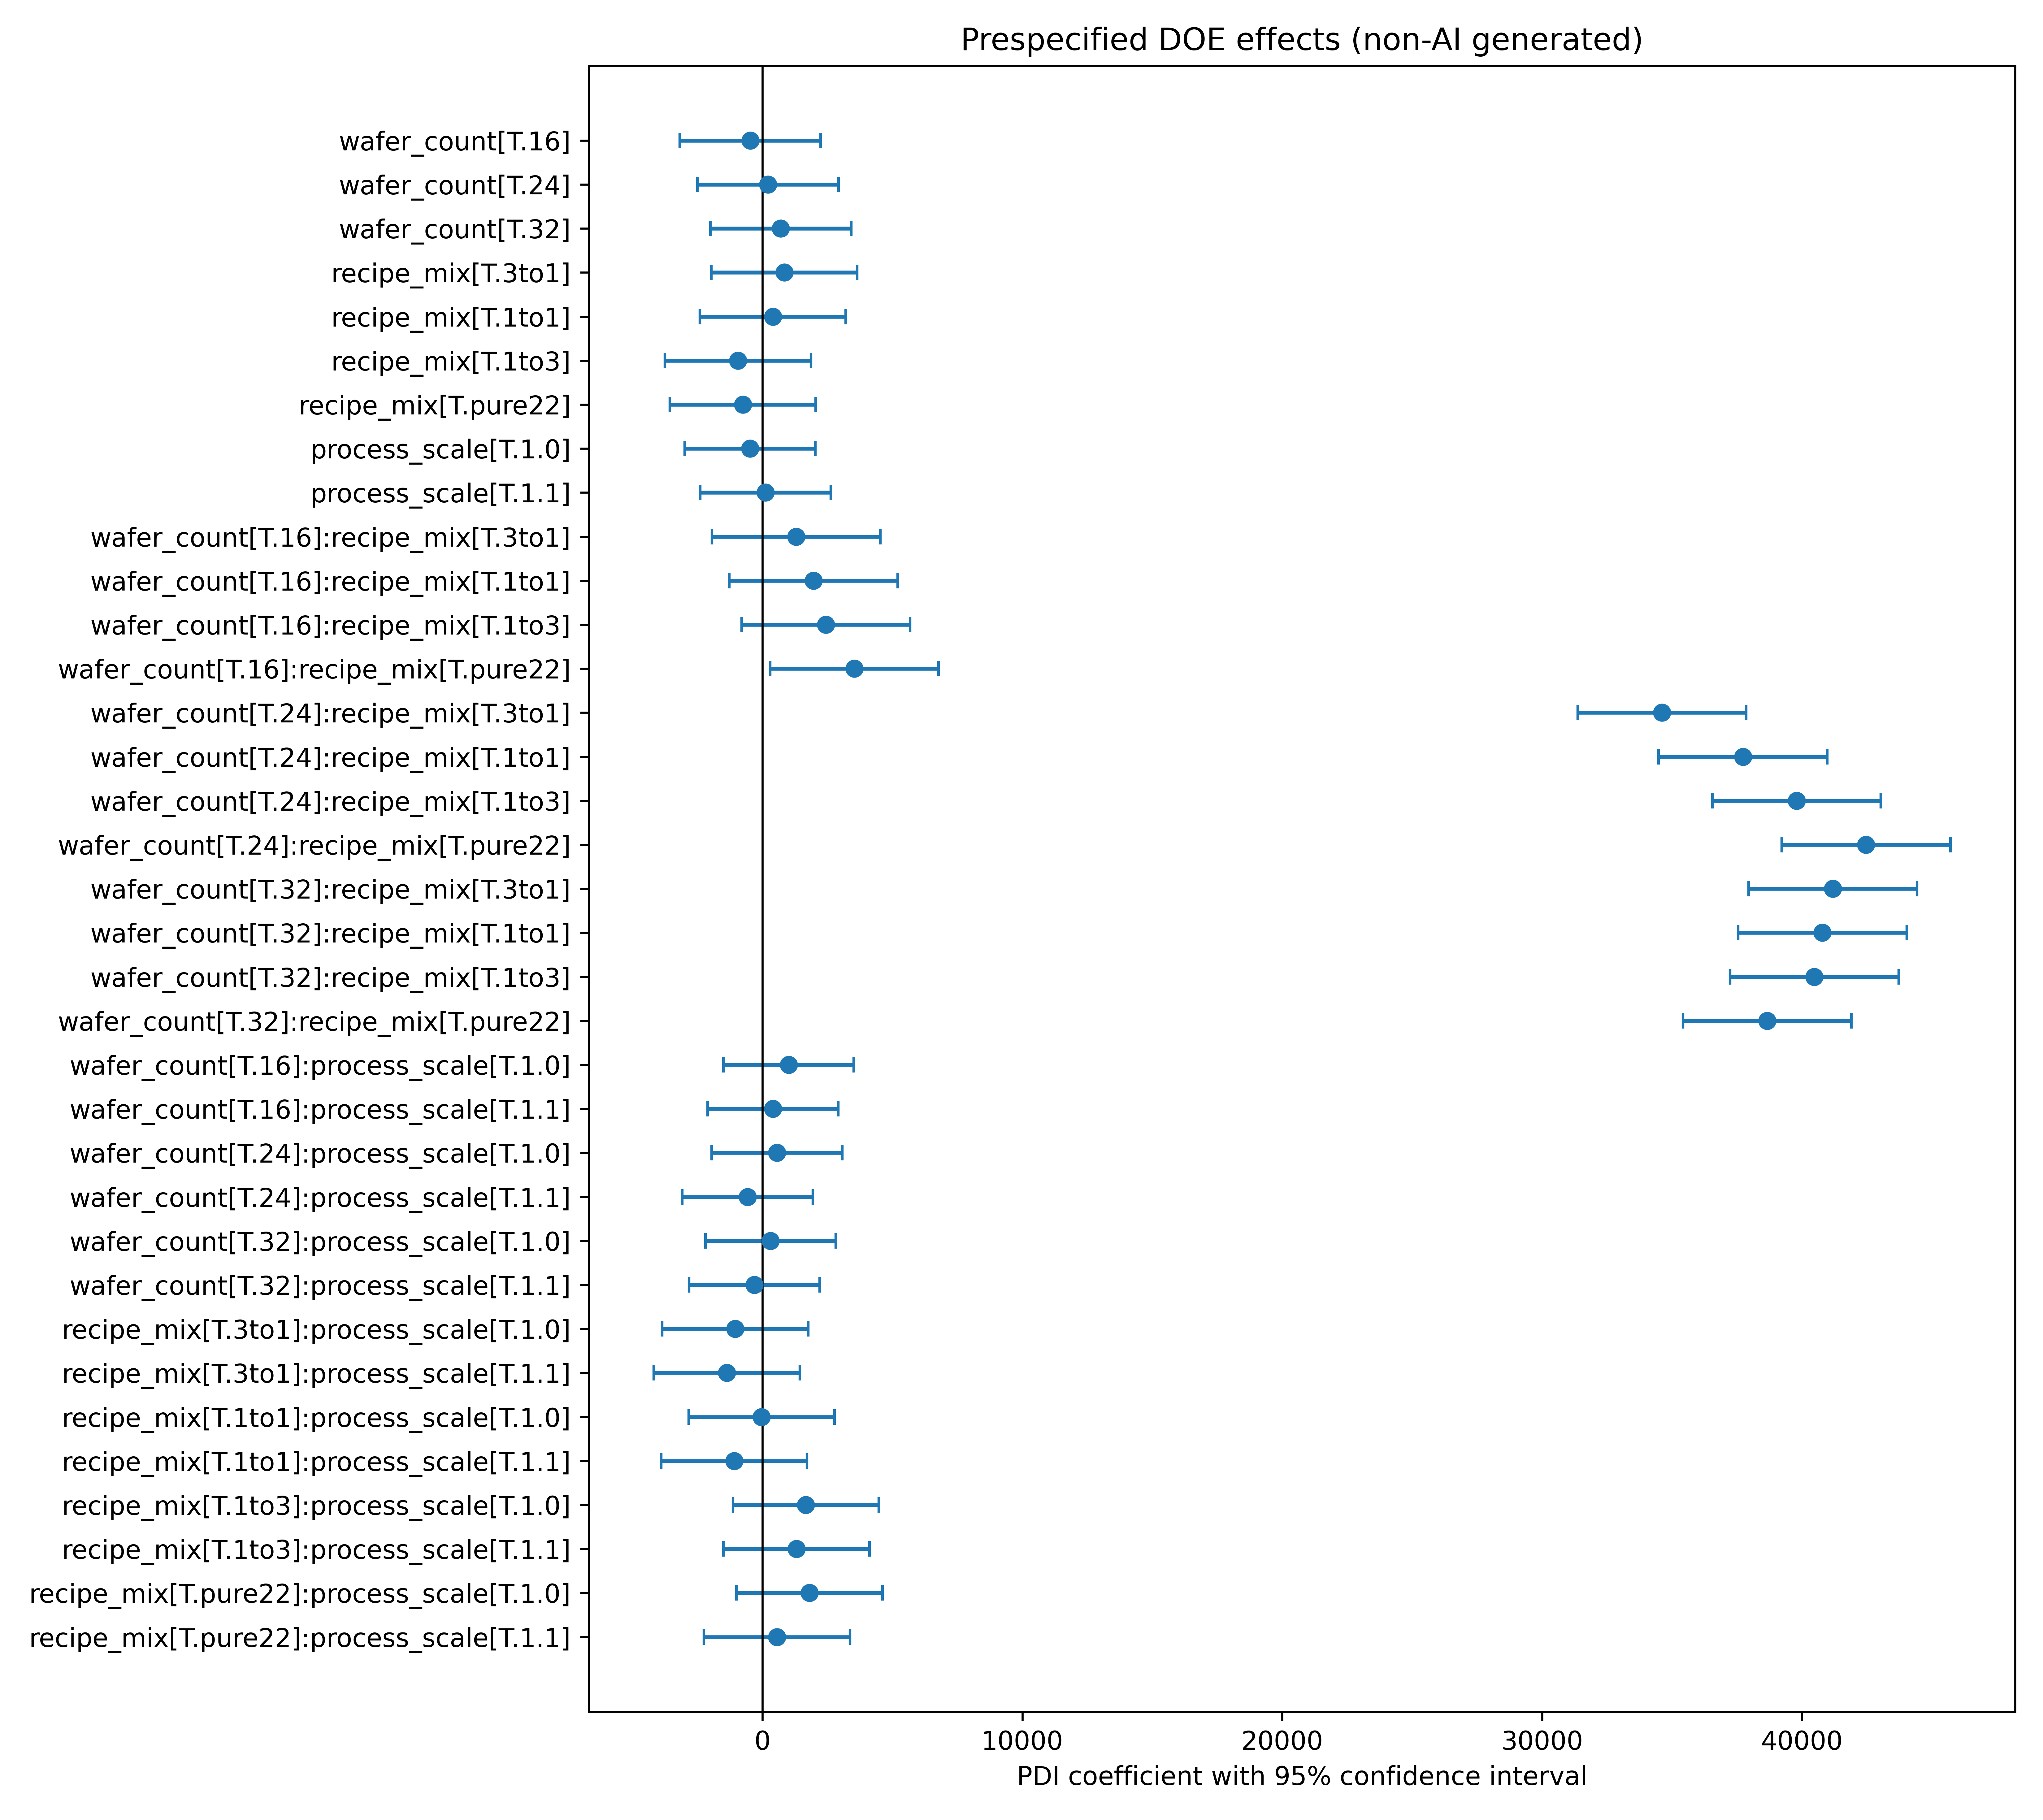
\includegraphics[width=0.96\linewidth]{Figure_DOE_PDI_effects.png}
\caption{PDI预设析因效应。点为OLS系数，误差线为95\%置信区间，竖线表示零。}
\label{fig:doe-zh-new}
\end{figure}

\subsection{敏感性验证预设扰动下的可运行性}

80次单因素敏感性运行全部返回经求解器检查的incumbent。较长清洗间隔对应最低平均
PDI（28899.41），较慢搬运对应最高平均PDI（42478.32）。该模式与较长清洗间隔减少
假片专用中断、较慢搬运收紧共享机械手时序相容，但单因素实验不能识别这两种机制的
因果作用。全部预设扰动下均保持可行排程交付；由于实验只包含默认SCIP一种方法，
它不支持跨方法稳健性排名。

\subsection{分布外压力实验验证规模扩展可行性}

分布外测试把批次扩大到40--64片并改变产品混流组成。729次运行全部获得保存解，
且均通过SCIP及针对同一MILP的后处理检查。由于全部运行均使用完整搜索窗口，表~\ref{tab:ood-zh-new}采用
PDI和终止gap区分求解轨迹。

\begin{table}[htbp]
\centering
\caption{分布外压力实验；统计量先在9个制造实例内聚合。}
\label{tab:ood-zh-new}
\resizebox{\linewidth}{!}{%
\begin{tabular}{lrrrr}
\toprule
方法 & 运行数 & 可行解率（\%） & 平均PDI & 平均gap（\%） \\
\midrule
SCIP & 27 & 100 & 73670.99 & 171.35 \\
自适应割选择 & 27 & 100 & \textbf{70915.54} & \textbf{160.78} \\
HEM-13D & 135 & 100 & 73003.59 & 165.88 \\
HEM-13D+Beam & 135 & 100 & 73165.58 & 167.04 \\
仅23维特征 & 135 & 100 & 74187.22 & 169.96 \\
结构补全+贪心 & 135 & 100 & 73507.76 & 168.54 \\
\method{} & 135 & 100 & 73919.15 & 170.02 \\
\bottomrule
\end{tabular}}
\end{table}

自适应割选择取得最低分布外PDI，\method{}的观察平均终止gap比默认SCIP低0.78\%。
全部分布外方法对比经全局Holm校正后均未达到显著。
完整结果区分出两类证据：\method{}在标称生产范围取得最低观察平均PDI，共享的
SPBS--MILP--SCIP求解链则在每次更大分布偏移运行中都交付了经求解器检查的可行排程。
七种方法均使用完整搜索窗口且没有证明分布外最优性，表明全局界闭合是极端规模下
仍需攻克的核心难点。

\subsection{工业启示}

完整证据给出三点工业启示。第一，在同一总预算内分层处理吞吐量和排程质量，与仅解
单阶段相比得到等待和节拍指标更低的保存排程；由于主求解预算分配不同，该差异属于
工作流证据。第二，预计算且经求解器检查的SPBS输入带来本文最大的显著求解窗口内PDI差异，
但端到端部署还应另计SPBS构造成本。第三，观察消融结果支持让学习表示对应可迁移的
MIP数学角色。束搜索效应的符号反转与其和角色表示之间的耦合一致，但该组件比较本身
既未检验统计交互，也未证明单个组件的因果贡献。

本文显式分离的状态、资源和时序层为在线到达、随机加工及模块故障追索提供后续扩展
接口，但当前结论限于离线有限批次和所测试构型。在此范围内，同预算两阶段工作流的
保存排程具有显著更低的配对等待与节拍指标，\method{}在比较方法中取得最低观察标称
平均PDI和时间。

\section{结论}

本文为双源混流旋转腔室组合设备建立模型与算法一体化框架。两阶段MILP统一表示
产品晶圆、可复用真空区假片、混合旋转配方、清洗、共享机械手、装载锁和驻留约束。
同模式产品采用规范配对并固定到规范腔室槽位，故本文不声称内生优化产品分组或腔室
侧面；第一阶段优化端到端最大完工时间，第二阶段保持其离散排程和最大完工时间并
优化时序质量。

相对采用600~s主求解的单阶段流程，采用540~s主求解加至多60~s精修的完整两阶段
流程，其保存排程的路线总等待、最大等待、节拍变异和节拍偏差分别低51.91\%、
68.89\%、39.70\%和94.05\%；这些是同总预算工作流差异，不是纯第二阶段因果量。
\method{}在完整2700次七方法比较中取得最低观察平均PDI和求解时间，但相对HEM和
SCIP的差异未达显著。把预计算SPBS输入SCIP后，求解窗口内PDI低26.19\%，可行解率
达到100\%；SPBS构造时间不在该比较内。析因实验在预设网格内显示规模与混流构成的
强交互关联。9个更大分布偏移构型的729次运行全部产生经求解器检查与后处理核查的可行解，但未
证明分布外最优性。

因此，在本文离线有限批次、规范配对和固定槽位的建模边界内，两阶段MILP提供吞吐量--
运行质量的分层优化机制，同预算两阶段工作流得到更低的保存排程运行指标；结构感知
学习增强分支割在本次标称比较中取得最低观察平均anytime性能。二者共同覆盖了双源
混流旋转腔室组合设备的一类集成调度情形。

\section*{利益冲突声明}
作者声明不存在可能影响本文工作的已知财务利益或个人关系。

\section*{数据与代码可用性}
支撑本文结果的数据、数学实例、训练模型和源代码可向通信作者合理申请。正式发表版
将给出永久公共归档地址。

\section*{稿件准备过程中生成式AI和AI辅助技术的声明}
在本文准备及相关软件开发过程中，作者使用OpenAI Codex辅助稿件结构组织与语言润色、
LaTeX一致性与文献元数据核查、软件实现与调试、实验流程和验证脚本编制，以及代码审查
与分析文字完善。该工具未用于生成实验观测、改动求解器输出、选择有利运行或决定署名。
研究问题、模型假设、实验设计、结果解释和投稿决定均由作者作出；作者逐项复核并按需
修改全部AI辅助输出，核验文献、公式、代码、数据、统计解释与最终文本，并对论文及
相关研究产物承担全部责任。

\bibliographystyle{elsarticle-harv}
\bibliography{rdmct_cie_references}

\end{document}
